
\documentclass[times, 10pt,twocolumn]{article} 
\usepackage{latex8}


\usepackage{graphicx,amsmath,comment,fullpage}
\newcommand{\igH}[1]{\includegraphics[height=.9\textheight]{#1}}
\newcommand{\igW}[1]{\includegraphics[width=.9\textwidth]{#1}}
\newcommand{\igWh}[1]{\includegraphics[width=.7\textwidth]{#1}}
\newcommand{\igWhalf}[1]{\includegraphics[width=.45\textwidth]{#1}}
\newcommand{\lda}{Latent Dirichlet Allocation}


\author{Abram Hindle and Michael Godfrey and Ric Holt \\
\{ahindle,migod,holt\}@cs.uwaterloo.ca\\
Software Architecture Group (SWAG)\\
University of Waterloo\\
}




%\title{Windowed Developer Topic Analysis}
\title{What's hot and what's not:\\Windowing developer topic analysis}

\usepackage{rotating}   
\begin{document}


\newcommand{\affaddr}[1]{#1}
\newcommand{\aemail}[1]{#1}
%\numberofauthors{5}
\author{
%\alignauthor
Abram Hindle\\
%\affaddr{David Cheriton School of Computer Science}\\
\affaddr{University of Waterloo}\\
\affaddr{Waterloo, Ontario}\\
\affaddr{Canada}\\
\aemail{ahindle@cs.uwaterloo.ca}
%\alignauthor
\and
Michael W. Godfrey\\
%\affaddr{David Cheriton School of Computer Science}\\
\affaddr{University of Waterloo}\\
\affaddr{Waterloo, Ontario}\\
\affaddr{Canada}\\
\aemail{migod@cs.uwaterloo.ca}
%\alignauthor
\and
Richard C. Holt\\
%\affaddr{David Cheriton School of Computer Science}\\
\affaddr{University of Waterloo}\\
\affaddr{Waterloo, Ontario}\\
\affaddr{Canada}\\
\aemail{holt@cs.uwaterloo.ca}
%\alignauthor
%\and
%Gregorio Robles\\
%\affaddr{GSyc}\\
%\affaddr{Universidad Rey Juan Carlos}\\
%\affaddr{Madrid}\\
%\affaddr{Spain}\\
%\aemail{grex@gsyc.escet.urjc.es}
}






\maketitle
\begin{abstract}

%   At different times, developers focus on different topics and tasks
%   during development.  These different topics and tasks might
%   be obvious to developers familiar with the project, but other
%   stake-holders, like managers, might be less aware of the topics of
%   development. Imagine the scenario where developers unexpectedly had to deal with
%   issues orthogonal to the features suggested, at the end of the
%   iteration a manager would wonder where all the effort went to.
%   Currently it is difficult for stake-holders to
%   audit what actually occurred and when certain features or topics
%   were focussed on. We propose a visualization of the
%   changing development topics over time. Our approach uses a topic
%   analysis tool like Latent Dirichlet Allocation (LDA) or Latent
%   Semantic Indexing (LSI). Instead of applying the tool to the
%   entire corpus we apply it to windows (periods) of the corpus. This allows us to
%   see the evolving stream of topics of development occurring
%   over time.
  


%   During different periods, developers focus on different topics and
%   different tasks during development. Stake-holders, such as managers,
%   not directly involved with the development might have less awareness
%   of the project and the topics and tasks that the developers are
%   focussed on.  Imagine the scenario where a manager is trying to
%   discover where all the developers' effort went after features have
%   not been implemented because the developers unexpectedly had to deal
%   with issues orthogonal to these features.  We propose to help
%   stake-holder understand the topics of development by extracting
%   topics from the descriptions of changes that programmers provide
%   when they make changes.  We leverage topic analysis tools such as
%   Latent Dirichlet Allocation (LDA) or Latent Semantic Indexing (LSI)
%   to analyze periods, such as months, within a project's
%   lifetime. Previous work applied LDA and LSI to
%   to a project's entire lifetime.  These tools associate
%   descriptions with independent topics extracted from these
%   descriptions.  We propose a visualization of changing development
%   topics over time that allows us to see the evolving stream of topics
%   of development occurring over time. We also show that windowed topic
%   analysis offers benefits compare to entire lifetime topic analysis
%   because of the independence of topics between windows.

% During different periods, developers focus on different topics and
% different tasks during development. Stake-holders, such as managers, who are
% not directly involved with the project's development might have less awareness of the
% project and the topics and tasks that the developers have focussed on.
% Imagine the scenario where a manager is trying to discover where all the
% developers' effort went after features have not been implemented because the
% developers unexpectedly had to deal with issues orthogonal to these
% features.  We propose to help stake-holders understand the topics of
% development by extracting topics from the descriptions of changes that
% programmers provide when they make commits.  We leverage topic analysis
% tools such as Latent Dirichlet Allocation (LDA) or Latent Semantic Indexing
% (LSI) to analyze periods, such as months, within a project's lifetime,
% whereas previous work applied LDA and LSI to to a project's entire lifetime.  These
% tools associate descriptions with independent topics extracted from these
% descriptions.  
% We propose a visualization of changing development topics
% over time that allows us to see the evolving stream of topics of development
% occurring over time. We demonstrate that windowed topic analysis offers
% benefits over entire lifetime topic analysis because of the
% independence of topics between windows.



As development on a software project progresses, developers will naturally
shift their focus between different topics and tasks many times.  Managers
and newcomer developers often seek simple ways of understanding what tasks
have recently been worked on and how much effort has gone into each; for
example, a manager might wonder what unexpected tasks occupied their team's
attention during a period when they were supposed to have been implementing
a set of new features.  Tools such as Latent Dirichlet Allocation (LDA) and
Latent Semantic Indexing (LSI) can be used to analyze check-in comments
over the entire lifetime of a project, and previous work on developer topic
analysis has leveraged these tools to associate commit log comments with
independent topics extracted from these commit log comments.  In this work, we use
LDA and LSI to analyze periods, such as months, within a project's lifetime
to create a time-windowed model of changing development topics.  We propose
a visualization of this model that allows us to explore the evolving stream
of topics of development occurring over time, and we demonstrate that
windowed topic analysis offers strong advantages over entire lifetime topic
analysis because of the independence of topics between windows.





%   In this lab report we seek to explore how topics shift over time in
%   the source control repository of a project. We analyze commit
%   comments, and even source code per revision per each time window and
%   extract the topics prevalent in that window. We expect that topic
%   sets will change over time and the change in topic sets indicate a
%   change in the focus of development. We suppose this could help us to
%   segment the revisions on the time line to discover parts of an
%   iteration. For topic extraction we use \lda (LDA).

\end{abstract}

\section{Introduction}

%?


% 

% In the presence of fine grained changes and detailed change-logs

% Developers topics the focus of develop

% many change-logs how to sort by change type

% interleaved changes relate similar changes

What happened in the previous maintenance or development iteration? What were the developers
working on? What was the developer in the next cubicle working on?
Which common topics and issues were dealt with in the current
release of the software? What were the topics of the previous release?
Given the requirements agreed to at the start of the iteration did our
developers work on them? What else did they work on?

Topic analysis, with respect to Software Control Systems (SCSs) such
as CVS, Subversion, Git etc., is potentially valuable as it has many
uses for various stakeholders and uses.  Imagine a development team
has agreed to implement some features at the start of an iteration. By
the end of the iteration only some of the agreed upon features are
implemented. The developers insist they were focusing solely on the
features agreed upon, but what actually happened? Topic analysis could
help by teasing out the distinct topics or focusses of the
developers. Perhaps the developers had to deal with issues.
Developers might have grouped those orthogonal changes into one of the
features they were working on, thus when asked about how their time
was spent the orthogonal changes would not be covered. This is the kind of underlying story that we
hope that windowed topic analysis can uncover. If windowed topic
analysis can discover important but overlooked topics, it can help
both developers and managers. Developer can see a summary of what
worked on, and managers can development.





Commits in SCSs are not necessarily consistent, they can have multiple
purposes, thus we hope that these multiple purposes manifest themselves as
topics interleaved within the commits.   Others have demonstrated that by
using powerful topic analysis techniques, such as Latent Semantic Indexing
(LSI) and Latent Dirichlet Allocation (LDA), can aid in separating topics
from these mixed comments. These topics often describe distinct ideas
that are interleaved throughout the development. A topic represents a
groups of commit comments that are related to each other by their
content.  In this case a topic is a set of tokens.


% We suppose this could help us to segment the revisions on the time
% line to discover parts of an iteration.

One use of topic analysis is to help us partition a project's
time-line into periods of developer focus. By breaking apart an
iteration into sets of topics and trends (topics which recur), we may
be able to recognize the underlying software development process from
these commits. Alternatively, we can determine what particular
maintenance task was being performed are a given time.

We propose to extend the use of common topic analysis techniques by
executing them over windows of documents over time. We hope by looking
at topic clusters during periods or windows over time we can identify
continuous effort on a select group of topics as well reflect topics
that were local to that period. Figure \ref{fig:lda} is an example of
the kind of visualization we want to automatically generate. We want
to see topics that are unique to a certain time period, displayed
across the time axis. Those topics that recur, or occur over a
larger period are plotted continuously. In our example we have
summarized each topic with a single word.

In this paper we explore how topics shift over time in the source
control repository of a project, using several open source database
systems as examples. We analyze commit comments per revision in each
time window and we extract the topics in that time window. We expect
that topics in each window will change over time and the similarities
and differences in these sets of topics will indicate both developer
focus and changes in developer focus.

Our contributions include:
\begin{itemize}
\item Demonstrating the value of windowed topic analysis using trends
\item Multiple visualizations topics and trends over time
\item An exploratory case study using these techniques on several open source database systems.
\end{itemize}


\section{Background}

We now define some terms that we will use in the rest of the paper: A
\emph{message} is a block of text written by developers. In this
paper, messages will be the CVS commit comments made when the user
commits changes to files in a repository. A \emph{word distribution}
is the summary of a message by word count. The word distribution will
be over all messages looked at but since most words will not appear in
a message, a word distribution is effectively a word count divided by
the message size. A \emph{topic} is essentially a set of words that
form a word distribution that is unique and independent within the set
of documents in our total corpus. One could think of a topic as the
center distribution of a group of messages. In this paper we often
summarize topics by their top 10 most frequent words in their word
distribution.  A \emph{trend} is a one or more similar topics which
recur over time.  Trends are particularly important, as they indicate
long-lived and recurring topics that may provide key insights into the
development of the project.

%\subsection{Intro to LDA}

In terms of clustering and finding topic distributions, Latent
Dirichlet Allocation (LDA)~\cite{944937} competes with Latent Semantic
Indexing
(LSI)~\cite{1421013,1374321,10.1109/ICPC.2007.13,10.1109/ICPC.2006.17},
probabilistic Latent Semantic Indexing (pLSI)~\cite{944937} and
semantic clustering~\cite{1698774,1566153}. These tools are used for
document modelling, document clustering and collaborative
filtering. What LDA attempts to do is encode documents as mixture
model of topics.  LDA is used in software engineering
literature~\cite{lukins2008,10.1109/MSR.2007.20,NIPS2007637,1321709}
is to extract topic clusters from documents such as methods, bug
reports, source code and files.

LDA, LSI and semantic clustering extract topic
clusters from the documents that are independent from one another. LDA
does not name these clusters but the clusters consist of words whose
relationship is often obvious to someone familiar with the corpus. We
could swap LDA for LSI or semantic clustering and produce similar
results. Our data is posed as documents with word distributions (word
counts per documents) and LDA extracts distinct topics (clusters of
words) from the documents.

\subsection{LDA, LSI and Semantic Clustering}

In order to infer or associate the expertise of an author with topics
extracted from SCS, Linstead et al. proposed an author-source-code model
using LDA~\cite{10.1109/MSR.2007.20,NIPS2007637,1321709}. This model
is essentially an extension of the author-topic (AT)
model~\cite{1036902}, which associated authors and topics extracted
with LDA.

Lukins, Kraft and Etzkorn~\cite{lukins2008} use LDA to help bug
localization by querying for documents that are related to a bug's topic. They
used LDA to build a topic model and then queried against it using
sample documents. These queries would indicate the proportion of
topics that were associated with the query and thus possible the
related documents.

LSI is related to LDA and has been used to identify topics in software
artifacts for formal concept analysis and concept
location~\cite{1421013,1374321,10.1109/ICPC.2007.13,10.1109/ICPC.2006.17}.
Concept analysis aims to automatically extract concepts from source
code or documents that are related to the source code.  Concept location concerns how
high level concepts relate to low level entities such as source code, for
example, when fixing a bug how and where do the concepts in the bug
report map back to the source code?  Semantic Clustering has also been
used for similar purposes~\cite{1698774,1566153} as it is similar to
LSI.

Grant et al.~\cite{scottcordy} have used an alternative technique,
 called Independent Component Analysis to
separate topic signals from software code. 

Our technique differs from the previous techniques because we apply
LDA locally to month-long windows of commit comments, where as other
approaches apply LDA once to the entire project. This allows us to
examine the time-based windowing of topics over its development
history.


%      1. [ ] LDA itself
%      2. [ ] Maletic stuff
%      3. [ ] WCRE: Scott/Jim
%      4. [ ] WCRE: Bug LDA stuff
%      5. [ ] MSR: Challenge work
%      6. [ ] FCA work
%4. [ ] Methodology [0/9]


\section{Preliminary Case Study}

In our first exploratory pass we wanted to see if LDA could provide
interesting topics extracted from a real system. We took the
repository of MySQL 3.23, extracted the commits, grouped them by 30
day non-overlapping windows, and then applied LDA to each of these
windows. We asked LDA to make 20 topics per window and we then
carefully examined the top 10 most frequent words in that topic.  We
found there were common words across topic clusters, such as
\emph{diffs}, \emph{annotate} and \emph{history}, these words probably should
be viewed as stop words. There were notable transitional topics such
as in the first window the word \emph{bitkeeper} appears because MySQL
adopted Bitkeeper for their source control system yet in the following
windows there were no mentions of Bitkeeper. \emph{RENAME} also only
appeared once in the first window and never again. Per each topic we
tried to identify the purpose of the topic; to our surprise we found
that even with onlyy a little familiarity with the code base that
naming the topic was straightforward.

A sub-sampling of the notable topic words is displayed in Table
\ref{tab:portability}.  To name the topics we selected terms that
seemed to best summarize those topics.  After viewing these topics, it was
obvious that we would have to combine try to track the evolution of
topics over the windows or rank topics by similarity, thus if they
were similar enough we joined them into a trend. Figure \ref{fig:lda}
displays a sample plot of the extracted topics in table
\ref{tab:portability}.

%It is apparent that we have to compare these topics some how by
%item-set or similarity.

% \begin{table*}
% \centering
% \begin{tabular}{|ccc|l|}
% \hline
% 2000 &  Jul &  31 &    chmod \\
% 2000 &  Sep &  29 &    fixes benchmark logging windows \\
% 2000 &  Nov &  28 &    typo fix insert\_multi\_value \\
% 2001 &  Jan &  27 &    fixes Innobase Cleanups auto-union \\
% 2001 &  Mar &  28 &    2 topics bugfix, logging , TEMPORARY,  \\
% \hline
% 2001 &  Jul &  26 &    update Allow TABLES LOCK [a] \\ 

% 2001 &  Aug &  25 &    tables row version [a] \\
% \hline
% 2001 &  Sep &  24 &    update checksum merge \\
% 2001 &  Oct &  24 &    fixed fix \\
% 2001 &  Dec &  23 &    HPUX SCO fix \\
% \hline
% 2002 &  Feb &  21 &    net buffer length  max\_allowed\_packet [b] \\
% 2002 &  Mar &  23 &    small buf fix [b]  \\
% \hline
% 2002 &  May &  22 &    [popular] fix SCO OSF1 table\_name \\
% 2002 &  Nov &  18 &    HPUX11 compiler HP \\
% \hline
% 2003 &  Feb &  16 &    Linux errno  [c] \\
% 2003 &  Mar &  18 &    alarm bookmark bug [c] \\
% \hline
% 2003 &  Sep &  14 &    Auto logging merge windows distribution fix 64-bit 4.0 Cleanup \\
% \hline
% \end{tabular}
% \caption{Tracking topics associated with the word portability, note some continuous blocks}
% \label{tab:portability}
% \end{table*}

\begin{table}
\centering
\begin{tabular}{|cc|l|}
\hline
2000 &  Jul &      chmod \\
2000 &  Sep &      fixes benchmark logging Win32 \\
2000 &  Nov &      fixes insert\_multi\_value \\
2001 &  Jan &      fixes Innobase Cleanups auto-union \\
2001 &  Mar &      bugfix logging  TEMPORARY  \\
\hline         
2001 &  Jul &      TABLES update Allow LOCK \\ 
               
2001 &  Aug &      TABLES row version \\
\hline         
2001 &  Sep &      update checksum merge \\
% 2001 &  Oct &      fixed fix \\
% 2001 &  Dec &      HPUX SCO fix \\
% \hline         
% 2002 &  Feb &      net buffer length  max\_allowed\_packet \\
% 2002 &  Mar &      small buf fix  \\
% \hline         
% 2002 &  May &      [popular] fix SCO OSF1 table\_name \\
% 2002 &  Nov &      HPUX11 compiler HP \\
% \hline         
% 2003 &  Feb &      Linux errno   \\
% 2003 &  Mar &      alarm bookmark bug \\
% \hline         
% 2003 &  Sep &      Auto logging merge windows distribution fix 64-bit 4.0 Cleanup \\
\hline
\end{tabular}
\caption{Sub-sampled topics from MySQL 3.23, some with continuous topics, these tokens were pulled from LDA topic. Each token is a summary of one LDA generated topic from MySQL 3.23 commit logs.}
\label{tab:portability}
\end{table}



\begin{figure*}
  \centering
  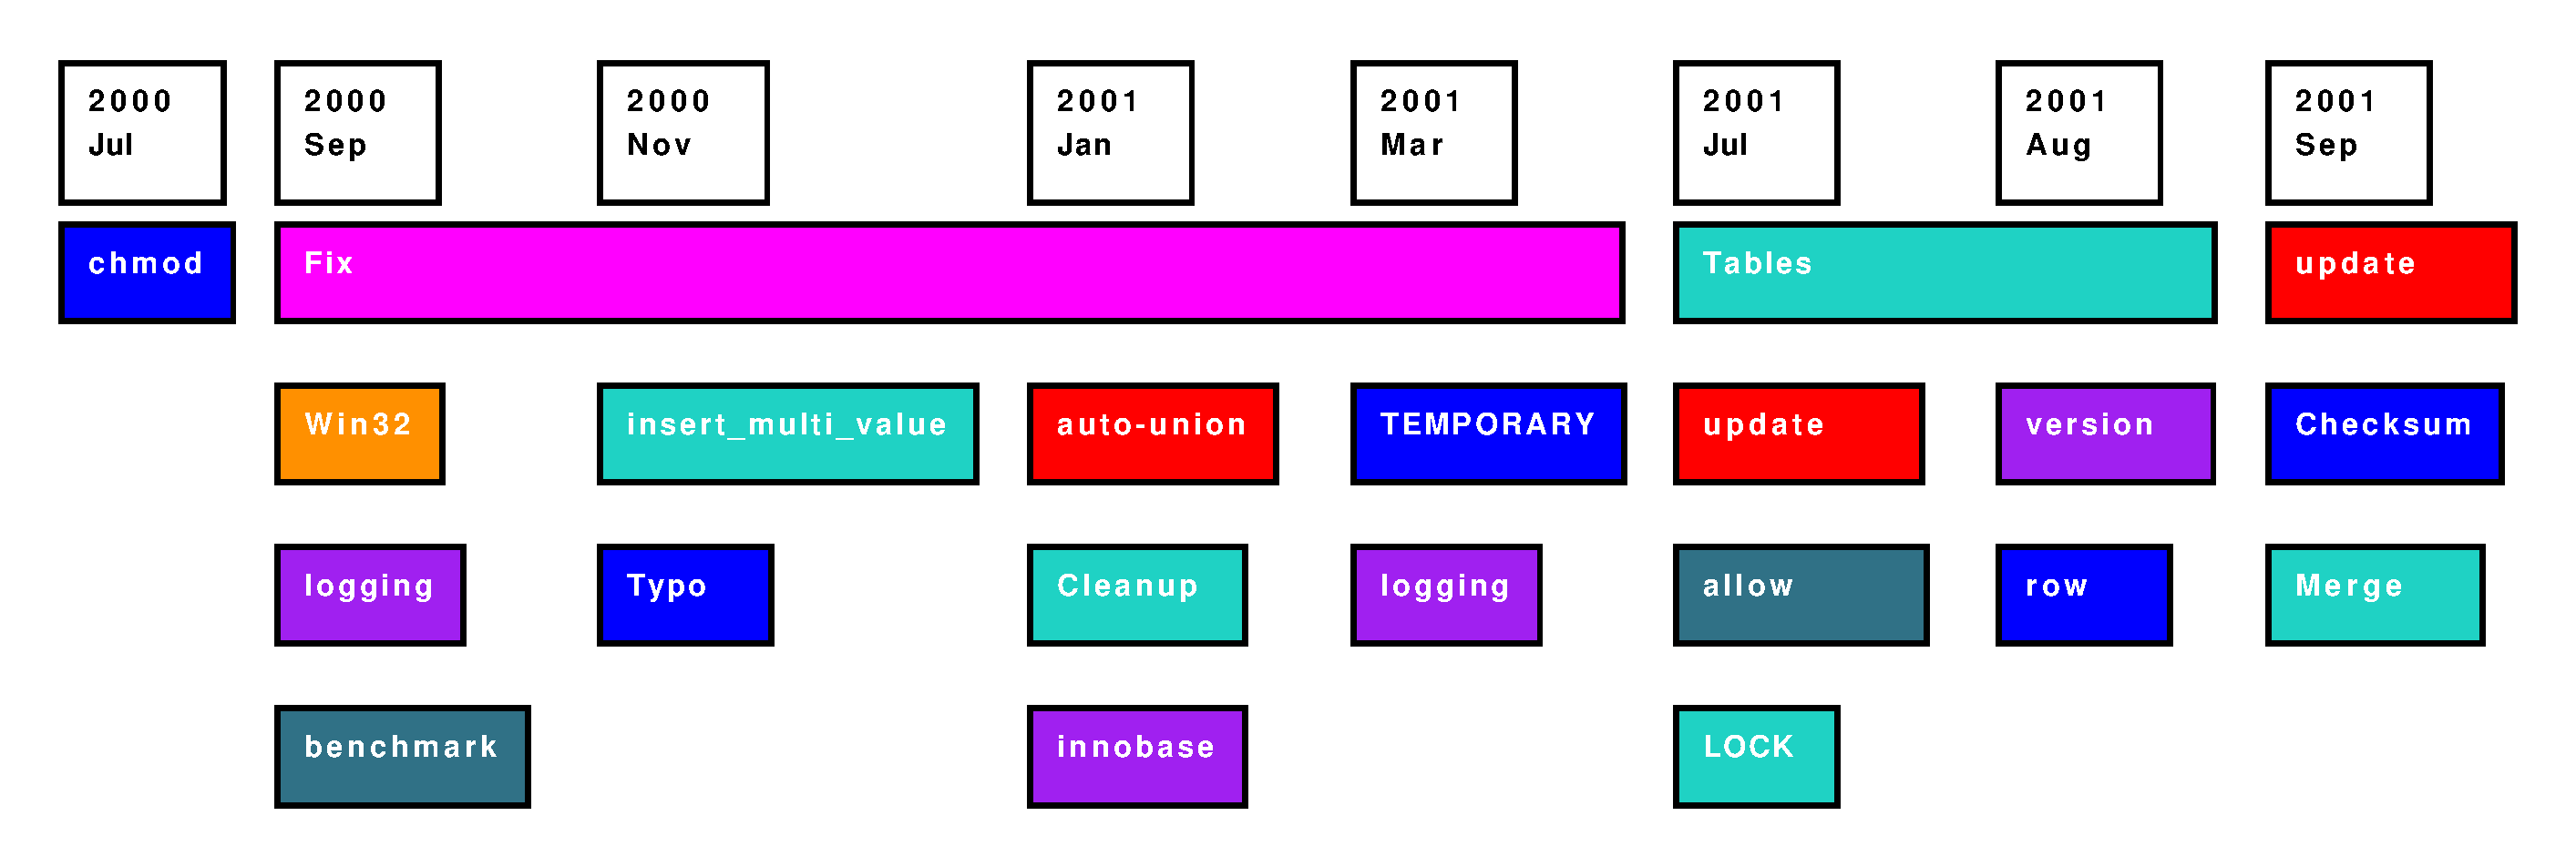
\includegraphics[width=0.9\textwidth]{lda}
  \caption{Example of topics extracted from MySQL 3.23. This is the kind of plot we eventually want to produce: named topics and topic trends. The horizontal axis is time in months and the vertical axis used to stack topics that occur at the same time. Longer topics are topics which recur in adjacent window. Colors are arbitrary.}
  \label{fig:lda}
\end{figure*}



\section{Methodology}
\begin{figure*}
  \centering
  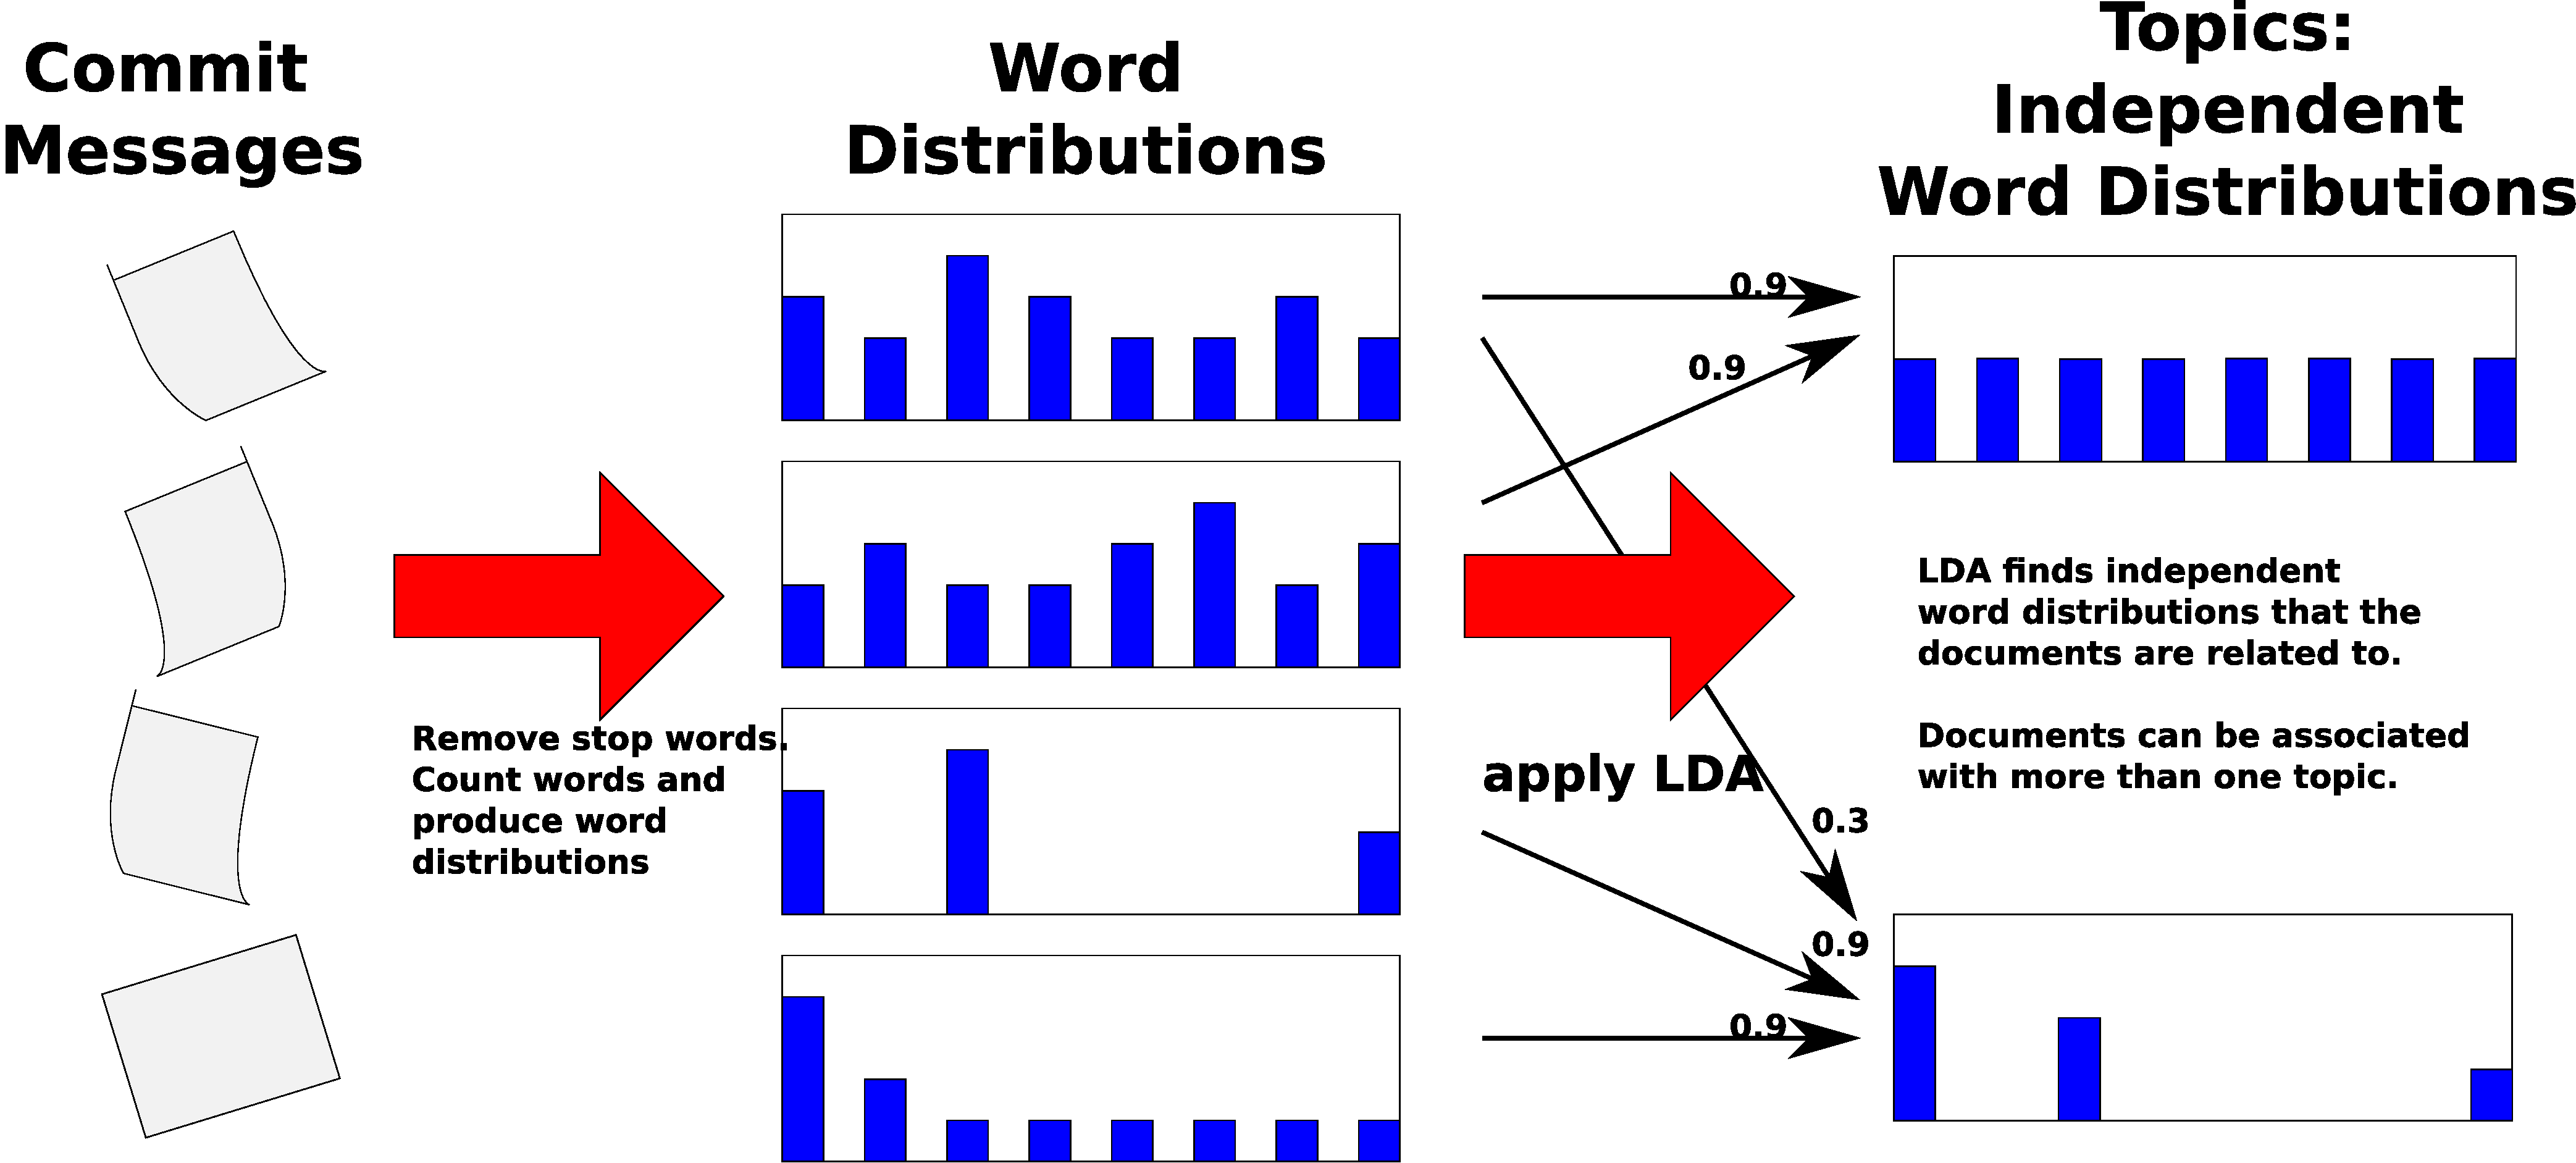
\includegraphics[width=0.9\textwidth]{commit-to-topics} 
  \caption{How commits are analyzed and aggregated into Topics and Trends. Commits are first extracted, then abstracted into word counts or word distributions. These word distributions are then given to topic clusterer like LDA which finds independent word distributions (topics) that these documents are related too and clusters or associates these documents with these topics.}
  \label{fig:commits}
\end{figure*}

Our methodology is to first extract the commits from SCS repositories such
as CVS or Bitkeeper. Then we extract the revisions and commits,
grouping the revisions into commits if necessary. We extract the
commit log message of each commit, count the occurrence of each word in
the message, remove stop words, and then produce word distributions
for each message.


\subsection{Extract Repositories}

We mirrored the repositories and their revisions using software such
as rsync, CVSSuck, \texttt{softChange} and bt2csv.
\texttt{softChange} provided a general schema for storing
revisions. CVSSuck and rsync mirrored CVS repositories while bt2csv
mirrored web accessible bitkeeper repositories.


%   2. [ ] Extract Documents
\subsection{Extract Documents}
%   3. [ ] Windowed Sets

The document we are analyzing are the changelog comments i.e., the comments that are added  when a revision to the source code is committed.
Documents are converted into word count distributions. These
distributions, which are then normalized by by the size of the
message. After all messages are processed the distributions are
extended to include all words in all distributions (each distribution
is extended with word bins of count 0).

\subsection{Windowed Sets}

Given all messages, we group the messages into windows. We could use
overlapping windows, but in this paper we use non-overlapping windows
of a set time unit because it simplifies analysis.  Windowing by time
allows for many levels of granularity. We usually used one month as
the length of our time windows, while we could use different
granularities for the study we think that a month is a sizable unit of
development, 4 weeks of development, which we consider to be fine
enough to show meaningful shifts but coarse enough not to show too
much detail.

\subsection{Apply Topic Analysis to each Window}

Once we have our data windowed, we apply our Topic Analysis tool to
each window and extract the top $N$ topic clusters, we used $20$
topics in our case study. Our Topic Analysis tool is an implementation
of LDA, but we could have used other similar tools like LSI, but
previous showed more promising topic analysis with LDA.

This is a very slow step as LDA takes a long time to run, and takes
even longer since we run it once per window. We note that this step is
a slow one, as executing even one instance of LDA involves significant
computation, and we perform LDA once per window.



%\subsection{Extract Clusters}


%   6. [ ] Cluster Similarity [0/1]
\subsection{Cluster Similarity}
%      1. [ ] need the tool
%             grab from the cluster analysis
%   7. [ ] Continuous Cluster Analysis


Once we have our topics extracted for each window, we analyze them and
look for repeating topics. We find repeating topics by comparing the
10 most common words of each topic.

We then abstract these topics by comparing them to each other.  Each
topic is compared to each other topic in the system, given a certain
threshold of top 10 similarity, such as 8/10 words. Then given this topic
similarity matrix, we find the transitive closure of similar topics;
that is, we fill flood along the similarity arcs until we have
partitioned the topics into clusters of similar topics. Figure
\ref{fig:closure} provides an example of clustering topics by the
topic similarity. These clusters of topics are called trends. A trend
is probably interesting and valuable if there is more than one topic in
the trend.

This technique has weaknesses in that nodes that are  a few neighbors away in
similarity might not share any similar words.  We do this because we
want to be able to color or highlight topics that are related to each
other and track them throughout time.

Once we have determined our similarity clusters we can choose to
analyze and to plot the topics.

\begin{comment}
Topic Clustering
 · Need to track continuous topics across
 · Similarity between topics
 · Clusters of the transitive closure of topics with X%
   similarity
    ­ Fill flood along similarity, make subsets of
      everyone who X% similar to any of their neighbors,
      make that a cluster
\end{comment}

\begin{figure}
  \centering
  \includegraphics[width=0.45\textwidth]{transitiveclosure}
  \caption{Topic similarity demonstrated by clustering topics by the transitive closure (connectedness)
    of topic similarity. Nodes are topics and
    arcs imply similarity. Similarity could be a measure such as
    topics share 8 out of 10 top ten words.}
\label{fig:closure}
\end{figure}



\subsection{Visualization}
%       1. [ ] need the visualizer

We have devised several ways to visualize these topics and
trends.  For all of these plots if we find trends that have continuous
segments, then we plot those segments as joined across time.  We have a
compressed stacked trend view, shown in Figure \ref{fig:topicsmear}
and Figure \ref{fig:zoomedsmear}, 
which displays trends as they occur
on the time-based x-axis (placement along the y-axis is arbitrary).
 Another plot we have is the trend-time line plot, shown in
Figure \ref{fig:trendtimeline}, each trend gets it own distinct y-value ,
while the x-axis is time; these topics are then each plotted on their
own line across time as they occur. Our final plot is the histogram
plot, shown in Figure \ref{fig:histogram} where we plot each trend on
its own line but stack up the segments of the trend, much like a plot
of counts or a histogram.


The first visualization is a compressed view
(Figure\ref{fig:topicsmear} and Figure \ref{fig:zoomedsmear}) where we
try to sink the larger trends to the bottom.  Once the larger trends
are stacked we fill in the gaps with the smaller trends in the same
window, and then stack the smaller trends on top.  Although there is a
chance that gaps will be left due to non-optimal stacking in practice
there are lot of small trends (90\% of all trends contain 1 topic)
which fill in these gaps quickly.  Different instances of the same
trend share the same colour; apart from that, the color of trends is
randomly chosen and color similarity is not meaningful.
The compressed view is convienant because it shows all of the
information and the repeating continuous trends are easy to pick out,
although repeating discontinuous trends are harder to spot.

The second visualization is the trend-time line plot (Figure
\ref{fig:trendtimeline}), it displays repeating trends more clearly by
dedicating a horizontal line for trend segments dedicated to one
trend. This means that if a trend contains discontinuous segments then the
segments appear on the same line. 
However, the least common trends need to be pruned away or the view will be cluttered with a lot of noise.

The third visualization is the histogram plot (Figure
\ref{fig:histogram}) which superficially resembles the time-trend
plot.  However, in this view the trends are plotted together by
stacking to their row so time information is lost, and the trends are
ordered by the number of topics in the trend.  The histogram plot
shows the count of instances of a trend and thus indicates which
trends occur the most. Unfortunately due to the large number of topics
given allotted space it is often best to crop off the trends with only
one topic, otherwise the tail is long.

%XXX Describe something useful like a trend
\begin{figure*}
  \centering
  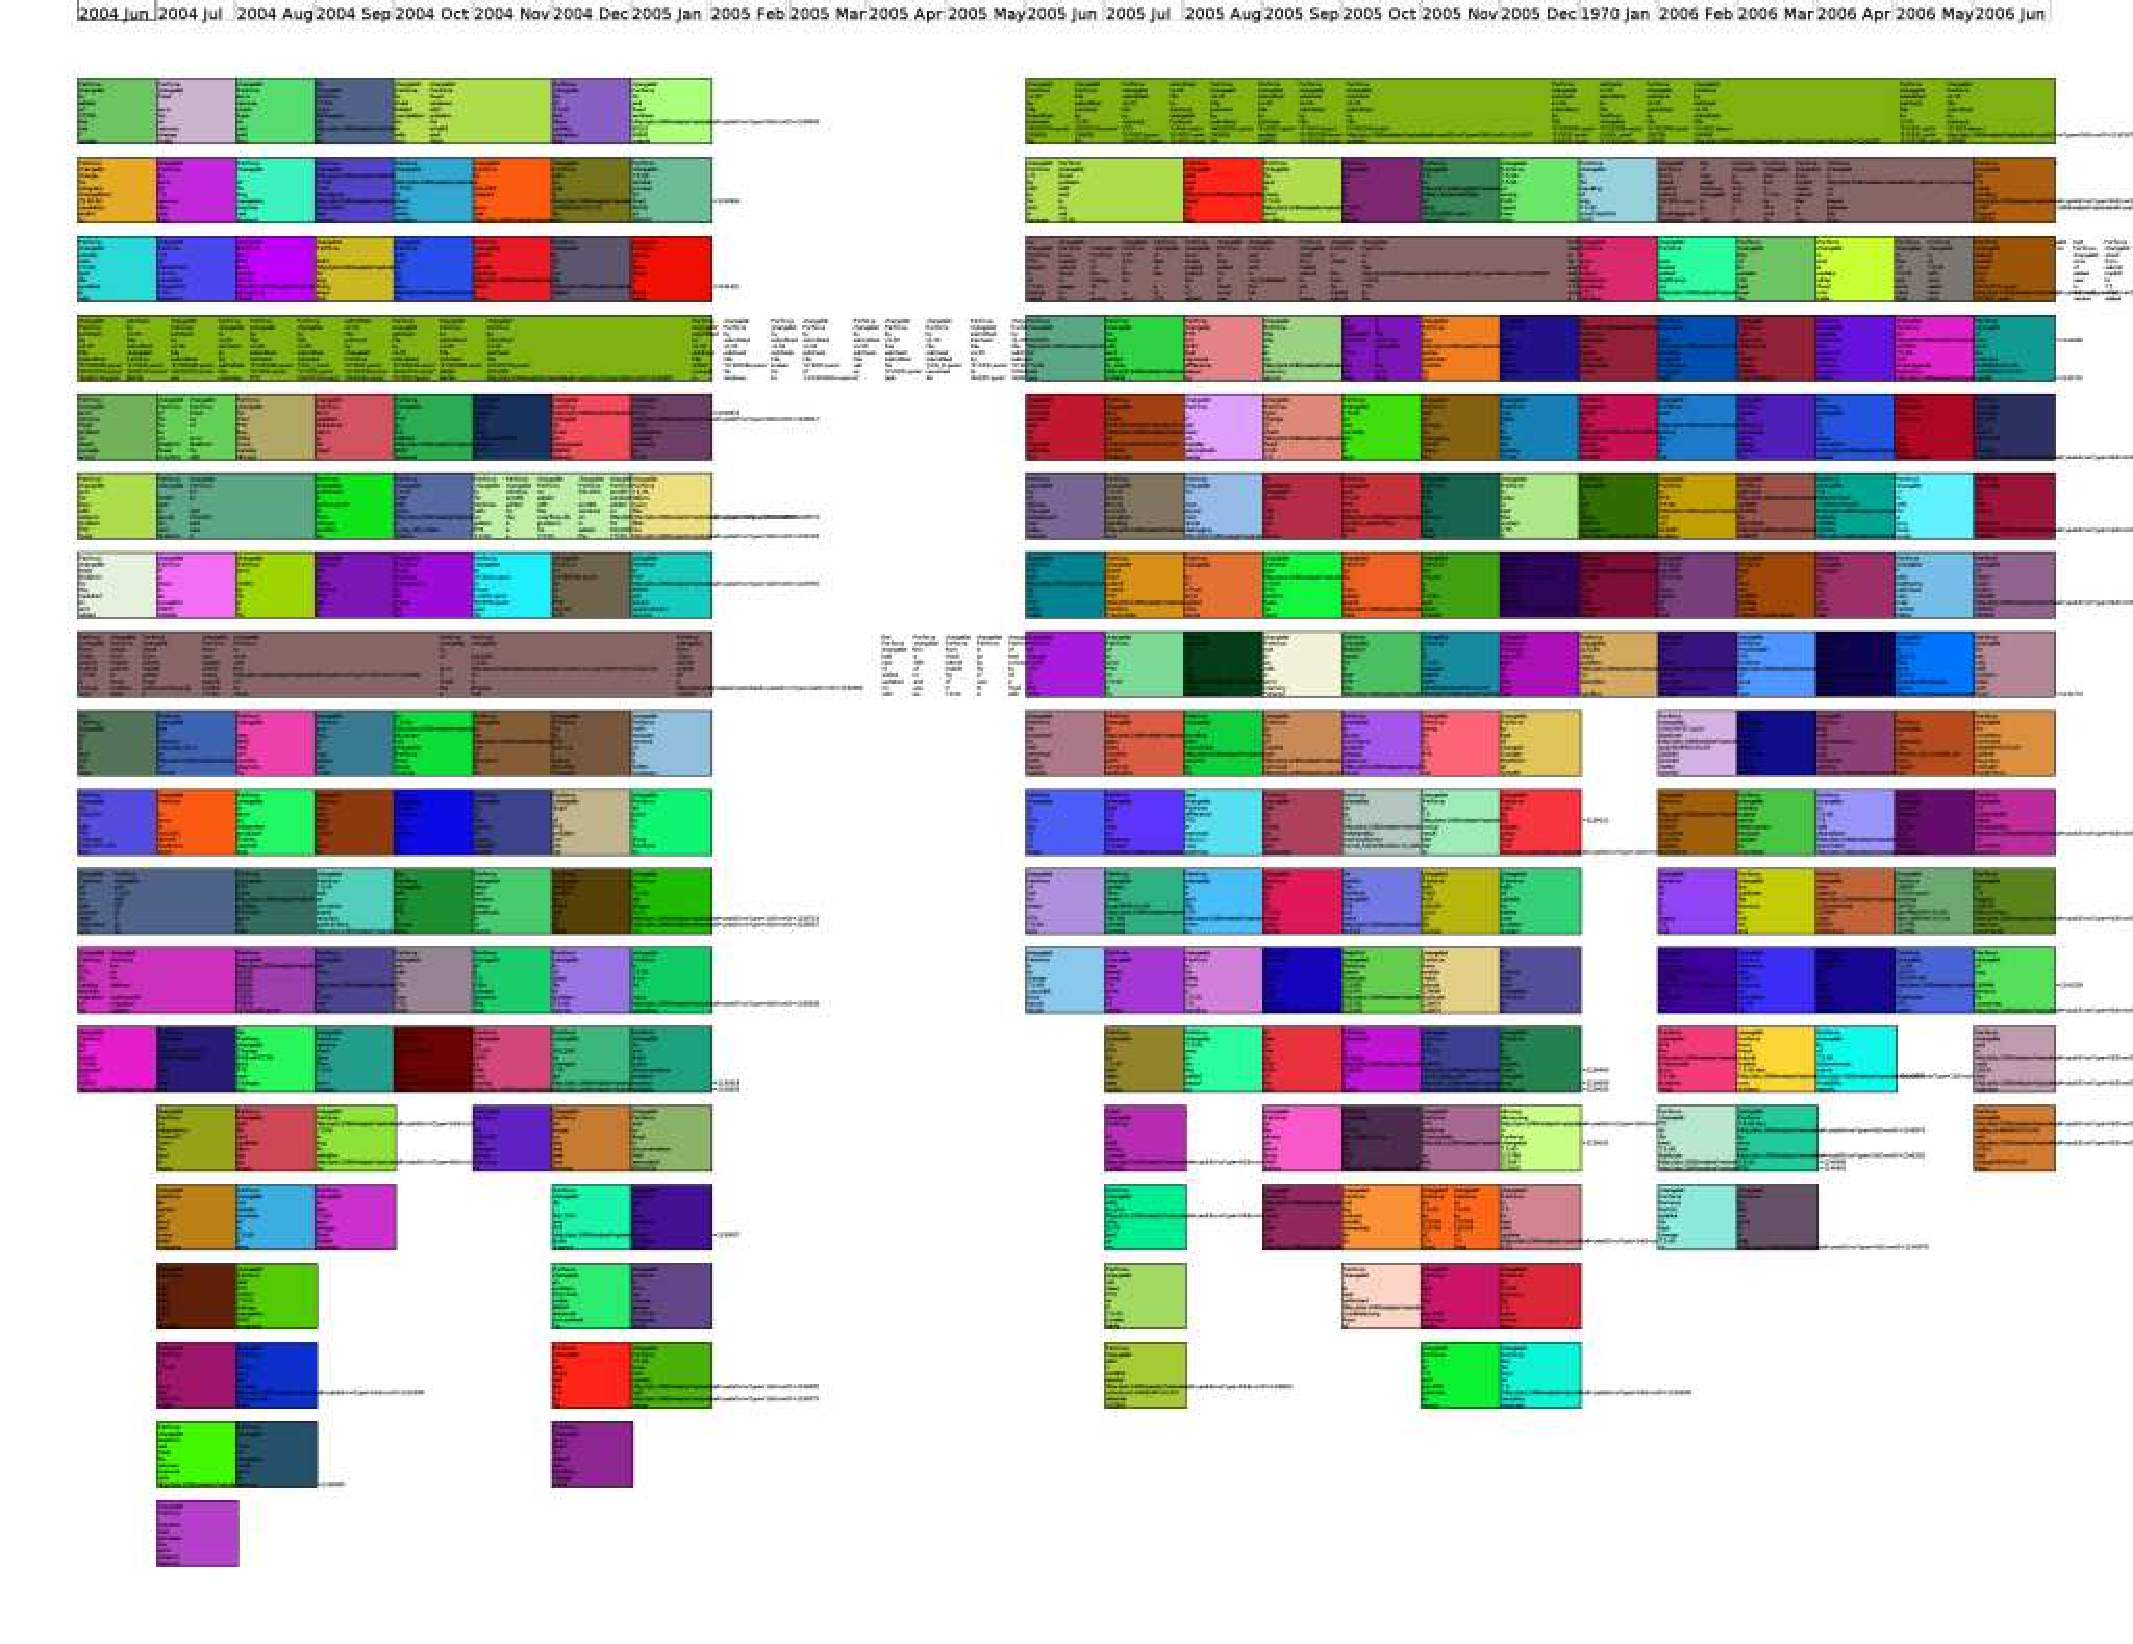
\includegraphics[width=1.0\textwidth]{fixed-time-smear-plot-scaled}
  \caption{Compact Trend Plot Topics per Month for MaxDB 7.500. The
    x-axis is time in months, the Y axis is used to stack topics
    occurring at the same time. Trends that are continuous are
    plotted as continuous blocks. The top 10 words in the topics are
    joined and embedded in box representing the topics.}
  \label{fig:topicsmear}
\end{figure*}


\begin{figure}
  \centering
  \includegraphics[width=0.45\textwidth]{fixed-time-smear-plot-cropped}
  \caption{Zoomed in Slice Compact Trend Plot of Topics per Month for MaxDB 7.500. The topic text is visible in each topic box. Trends are plotted across time continuously.}
  \label{fig:zoomedsmear}
\end{figure}


\begin{figure}
  \centering
  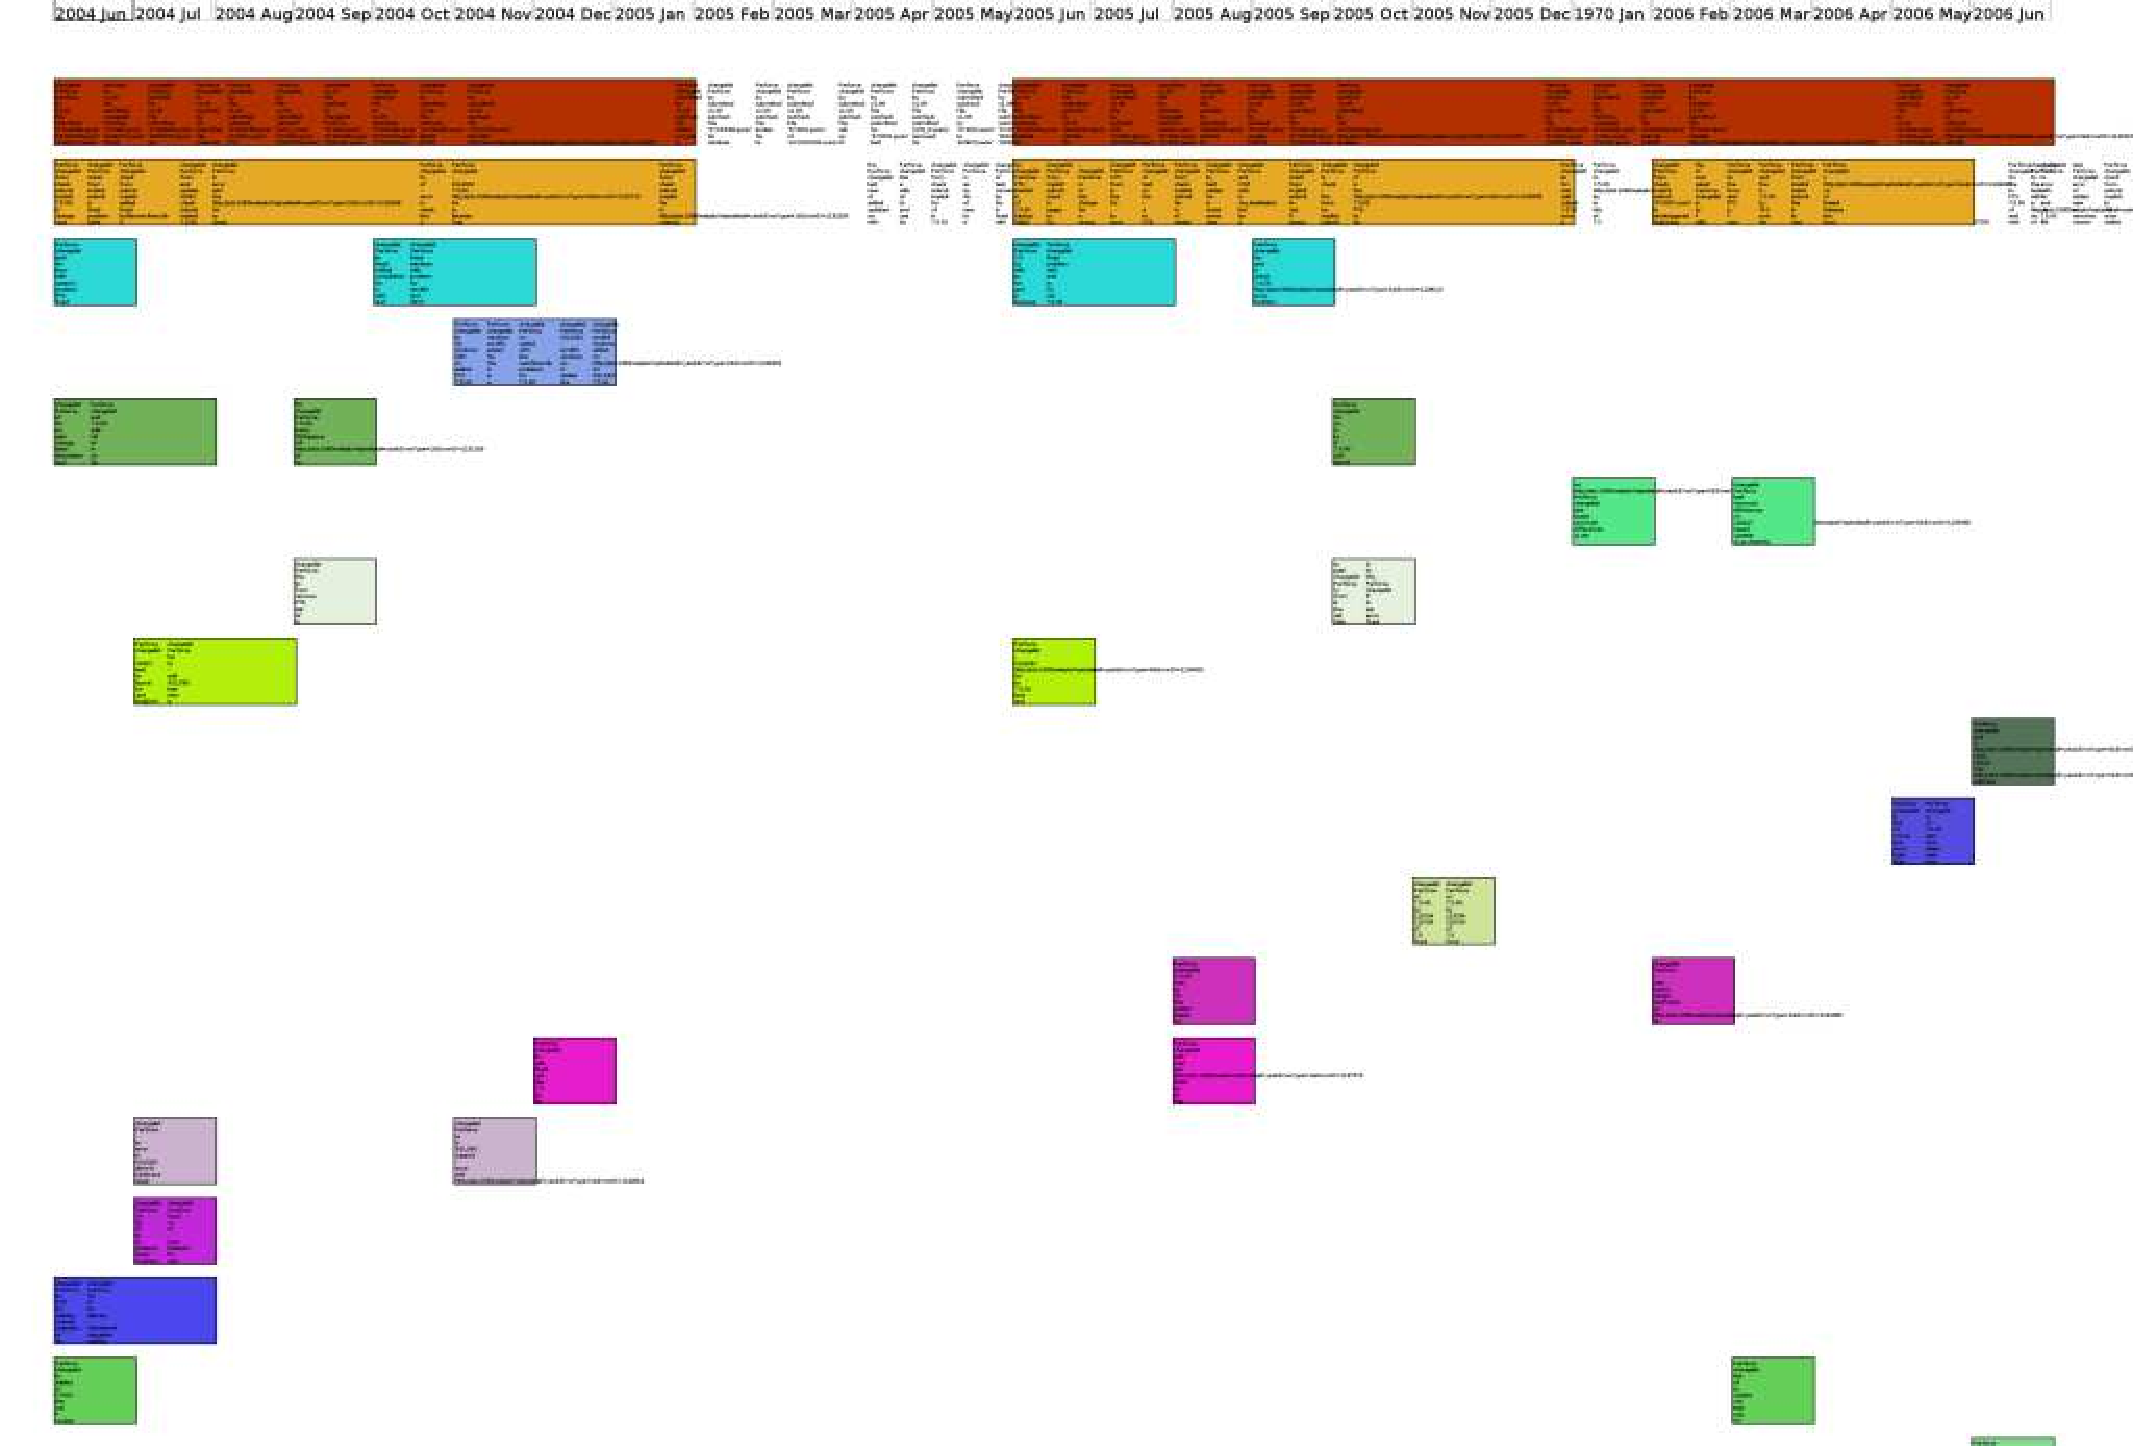
\includegraphics[width=0.45\textwidth]{class-smear-plot-crop-scaled}
  \caption{Trend-time Line: Trends plotted over time of MaxDB 7.500. Time in months are plotted along the x-Axis, each row on the y-axis is associated with a trend ranked by size in descending order}         
  \label{fig:trendtimeline}
\end{figure}


\begin{figure}
  \centering
  \includegraphics[width=0.45\textwidth]{histogram-cropped-scaled}
  \caption{Top part of trend histogram, ordered by topic occurance for MaxDB 7.500. X axis determines the number of continuous months of a trend. Trends are ranked  by the number of topics that a trend contains in descending order.}       
  \label{fig:histogram}
\end{figure}


\subsection{Datasets and Tools}

To extract data from CVS and BitKeeper we used softChange to extract
CVS repositories and provide a schema for our revision data. We used
bt2csv to extract BitKeeper revisions from BitKeeper web repositories.

We extracted the repositories of: PostGreSQL, MaxDB and
Firebird.

% Extractors:
% \begin{itemize}
% \item CVSSuck - CVS Suck mirrors RCS files from a CVS repository. 
% \item softChange - extract CVS facts to a PostgreSQL database.
% \item bt2csv - Convert BitKeeper repositories to facts in CSV
%   databases.
% \end{itemize}

Our analysis tools consisted of: Hiraldo-Grok, an OCaml-based variant
of the Grok query language; Gnuplot, a graph plotting package; lda-c,
a LDA package implemented by Blei et al. \cite{944937}; and our topic plotter, implemented
in Haskell.


%   1. [ ] LDA

%   2. [ ] Extractor

%   3.   Similarity

%   4.   Smearing

%   5.   Visualizer




%LDA Skeleton
%1. [ ] Abstract 
%2. [ ] Introduction

%3. [ ] Previous Work [0/2]
%   2. [ ] LDA Work [0/6]




\section{Results}

We applied our tools and visualizations to the repositories of several
open source database systems: PostgreSQL, MaxDB and Firebird.

%   1. Interesting smears 
%   2.   postgresql


%\subsection{MySQL}
%XXX DO MYSQL?

\subsection{Postgresql}
%   3.   mysql

%XXX Redo?

When we examined PostgreSQL, we did not find many trends with two or more topics; however, we did find one large trend which stretched across most of its existence.
 Much of the large trend consisted of stop words but it did
include topics which had non-stop words such as \emph{patch}, \emph{fix}, \emph{update}.

The second largest topic was interesting because it concerned changes from
1998, from developers using Central Europe Time (CEST), where the two
notable tokens were 1998 and CEST. These changes appear to be patches
submitted by one particular developer who lived in that timezone.

The third largest trend we found appeared to concerned with copying
and moving files between branches as it referenced the old branch.
branches.  We inferred this trend based on the fact that the old
version identifier was referenced, and we know this this is common
practice when performing a branch merge, since CVS cannot record such
information directly.


Once stop words were removed the some of the purposes became more
clear. The large trend disappeared, the largest trend became bug fixes
submitted by a developer named Dal Zotto which is a short trend.


%XXX REDO POSTEGRESQL?
% Large Trends is not the point!!!
% That's what normal LDA gives us

%But large trends are not the point, by investigating windowed trends
%we want more local information about trends being worked on.

\subsection{Firebird}
%   5.   what's that other db?

%XXX REDO?

We tracked Firebird from August 2000 to January 2006.
Our first attempt with Firebird resulted in a set of trends that were
dominated by one large trend containing tokens that were mostly stop
words such as references to one author
\texttt{carlosga05} and the words: \emph{the, to, a, for, of, is, it}.

The second largest trend related to branching and possibly merging; it
contained language such as ``was added on branch'' and contained
references to tags and branches.

The third largest trend contained references to the changelog, the
build system, architecture and platform support. It specifically
mentioned tokens such as \emph{Solaris}, \emph{port} and \emph{x86}.

Other trends included topics regarding AIX PPC compilation, updating
the build process, internationalization and UTF8, Darwin build support
and bug fixing.

Topics that were not trends but appeared to be  interesting were mostly external bug
fixes submitted to the project.
 In these cases, the developers would express thanks in their changelog comments, such as ``Thanks, Bill Lam''.  Other easily discernible topics included 
 tokens and topics such as: \emph{compiler workarounds}, \emph{nightly updates}, \emph{packets} and \emph{MSVC++}.

\subsection{MaxDB 7.500}

%XXX REDO?

%XXX Migod todo
% I think that you should enlarge this discussion of MaxDB (at the
% expense of the other systems) and make careful references to how the
% diagrams give you extra info about the evolution of the system (in
% terms of topics).

% We are trying to argue that (a) the approach is more informative that
% the naive static approach and (b) the diagrams are useful.



The plots we produced of MaxDB 7.500 were 
unlike those of the other systems, as 
 there was a
period where no real development occurred and thus there were no topics or trends
whatsoever. We have two periods to evaluate for MaxDB 7.500, the first
period from June 2004 to jan 2005, and the second period from June
2005 to June 2006.

The largest common trend has references to build system files like
SYSDD.punix and MONITOR.punix etc. Other tokens mentioned are Sutcheck
v1.09, the prefix SUT stands for Storable Unit Type. Sutcheck would
also automate check-ins using a Perforce SCS tool.

The second largest common trend seems to be a side effect of an
automated check-in which is annotated as ``implicit check-in''. These
were check-ins that were produced when importing changes from an
external Perforce repository.

The third most common trend, seen on Figure \ref{fig:trendtimeline}, seemed to
include tokens related to operating system support, such as Linux and
Windows, as well as architecture support, AMD64 and Opteron. The word
problem was common among all of those trends. This trend seemed
related to the smaller fourth largest trend which occurred nearby it
that had AMD64 and Windows tokens.


%XXX Edit
% Was reading lda.report
Bug tracker URLs dominated unique topics during some months. For
instance in the last month of MaxDB 7.500 development every topic
contained 1 unique Bug tracker URL, this pattern did not occur in the
previou month. We investigated the actual revisions and we did find
there was difference in behaviour between and that the last month of
development commits were mostly referencing the bug tracker. If the
topics of one month were 20 or more unique bug tickets being
addressed, the global LDA analysis would probably miss this, yet these
bug tickets were the focus of development for that month and not
necessarily globally relevant.

The query optimizer was a topic which recurred multiple times during
MaxDB's development. In our plots, topics which mention optimizer
occur four times yet in the large static plot (Figure
\ref{fig:statictopics}) it is not in any of the topics. A query
optimizer is rather important to an DBMS, but as we've shown it just
doesn't pop up as a topic on its own. We tried to remove words to see
if we could get optimizer topic out, after removing stop words and
then two of the most common words the global analysis finally had a
topic with optimizer in its topic ten words. This shows that optimizer
was important but it had been obscured, while it would have been
noticed using a more locally relevant approach that we propose.

We noticed that Perforce and Changelist were in just about every
topic, so we added them to the stop words list. Longer trends were
shortened and in some cases the total number of topics found per month
was less. Evaluating different similarity thresholds showed that by
removing common words one reduces the general similarity of topics,
that said the larger topics still existed. Thus if you add more
relevant stop words one should tune your topic similarity parameters
to handle this change.




\subsection{Compare to topics over entire development}

%XXX Migod notes This section is perhaps the most important of the
% whole paper.  You need expand it.  Maybe you should move the first
% two paras of the conclusions in here too.

% The thing that is most disappointing is that the argument is entire
% qualitative.  Can you give examples to make this sound less
% hypothetical?

% Can you add numbers in here to make the argument stronger?


Previous work on topic analysis that employed LSI and LDA typically
extracted a certain number of topics and tracked them over time. This
means that a single, static set of topics was tracked across the whole
development history of a project. 

We attempted the same kind of analysis, as shown in
Figure~\ref{fig:statictopics}. We extracted 20 topics and then plotted
the number of messages per month that were related to that topic. We
found was that one topic would often dominate the results, while
messages related to other topics did not appear very often.
% This technique seems useful if the 20 extracted topics are relevant
% and useful, that said one weakness of this approach is that documents
% for a topic might only occur in one time window, yet we are tracking
% messages that could be related to it over the entire lifetime of the
% project.
This approach seems reasonable if most of the extracted topics are of
broad interest during most of the development process.  However, it
may be that some topics are of strong interest but only briefly; in
such a case, a window-based model gives a much stronger indication of
the fleeting importance of such topics, and can help to put such a
topic into its proper context.

XXX Numbers and more argument

Even with our liberal topic similarity metrics that produced both
long and short trends, we showed that there are only a few trends in a
repository which recur. Since so few trends recur and so many
trends appear only once this suggests that global topic analysis might
be ignoring locally unique topics. 

The utility of global topic analysis is questionable if the value of
information decreases as it becomes older. Perhaps older trends will
dominate the topic analysis. Windowed localized topic analysis show
what are the unique topics.




\begin{figure}
  \centering
  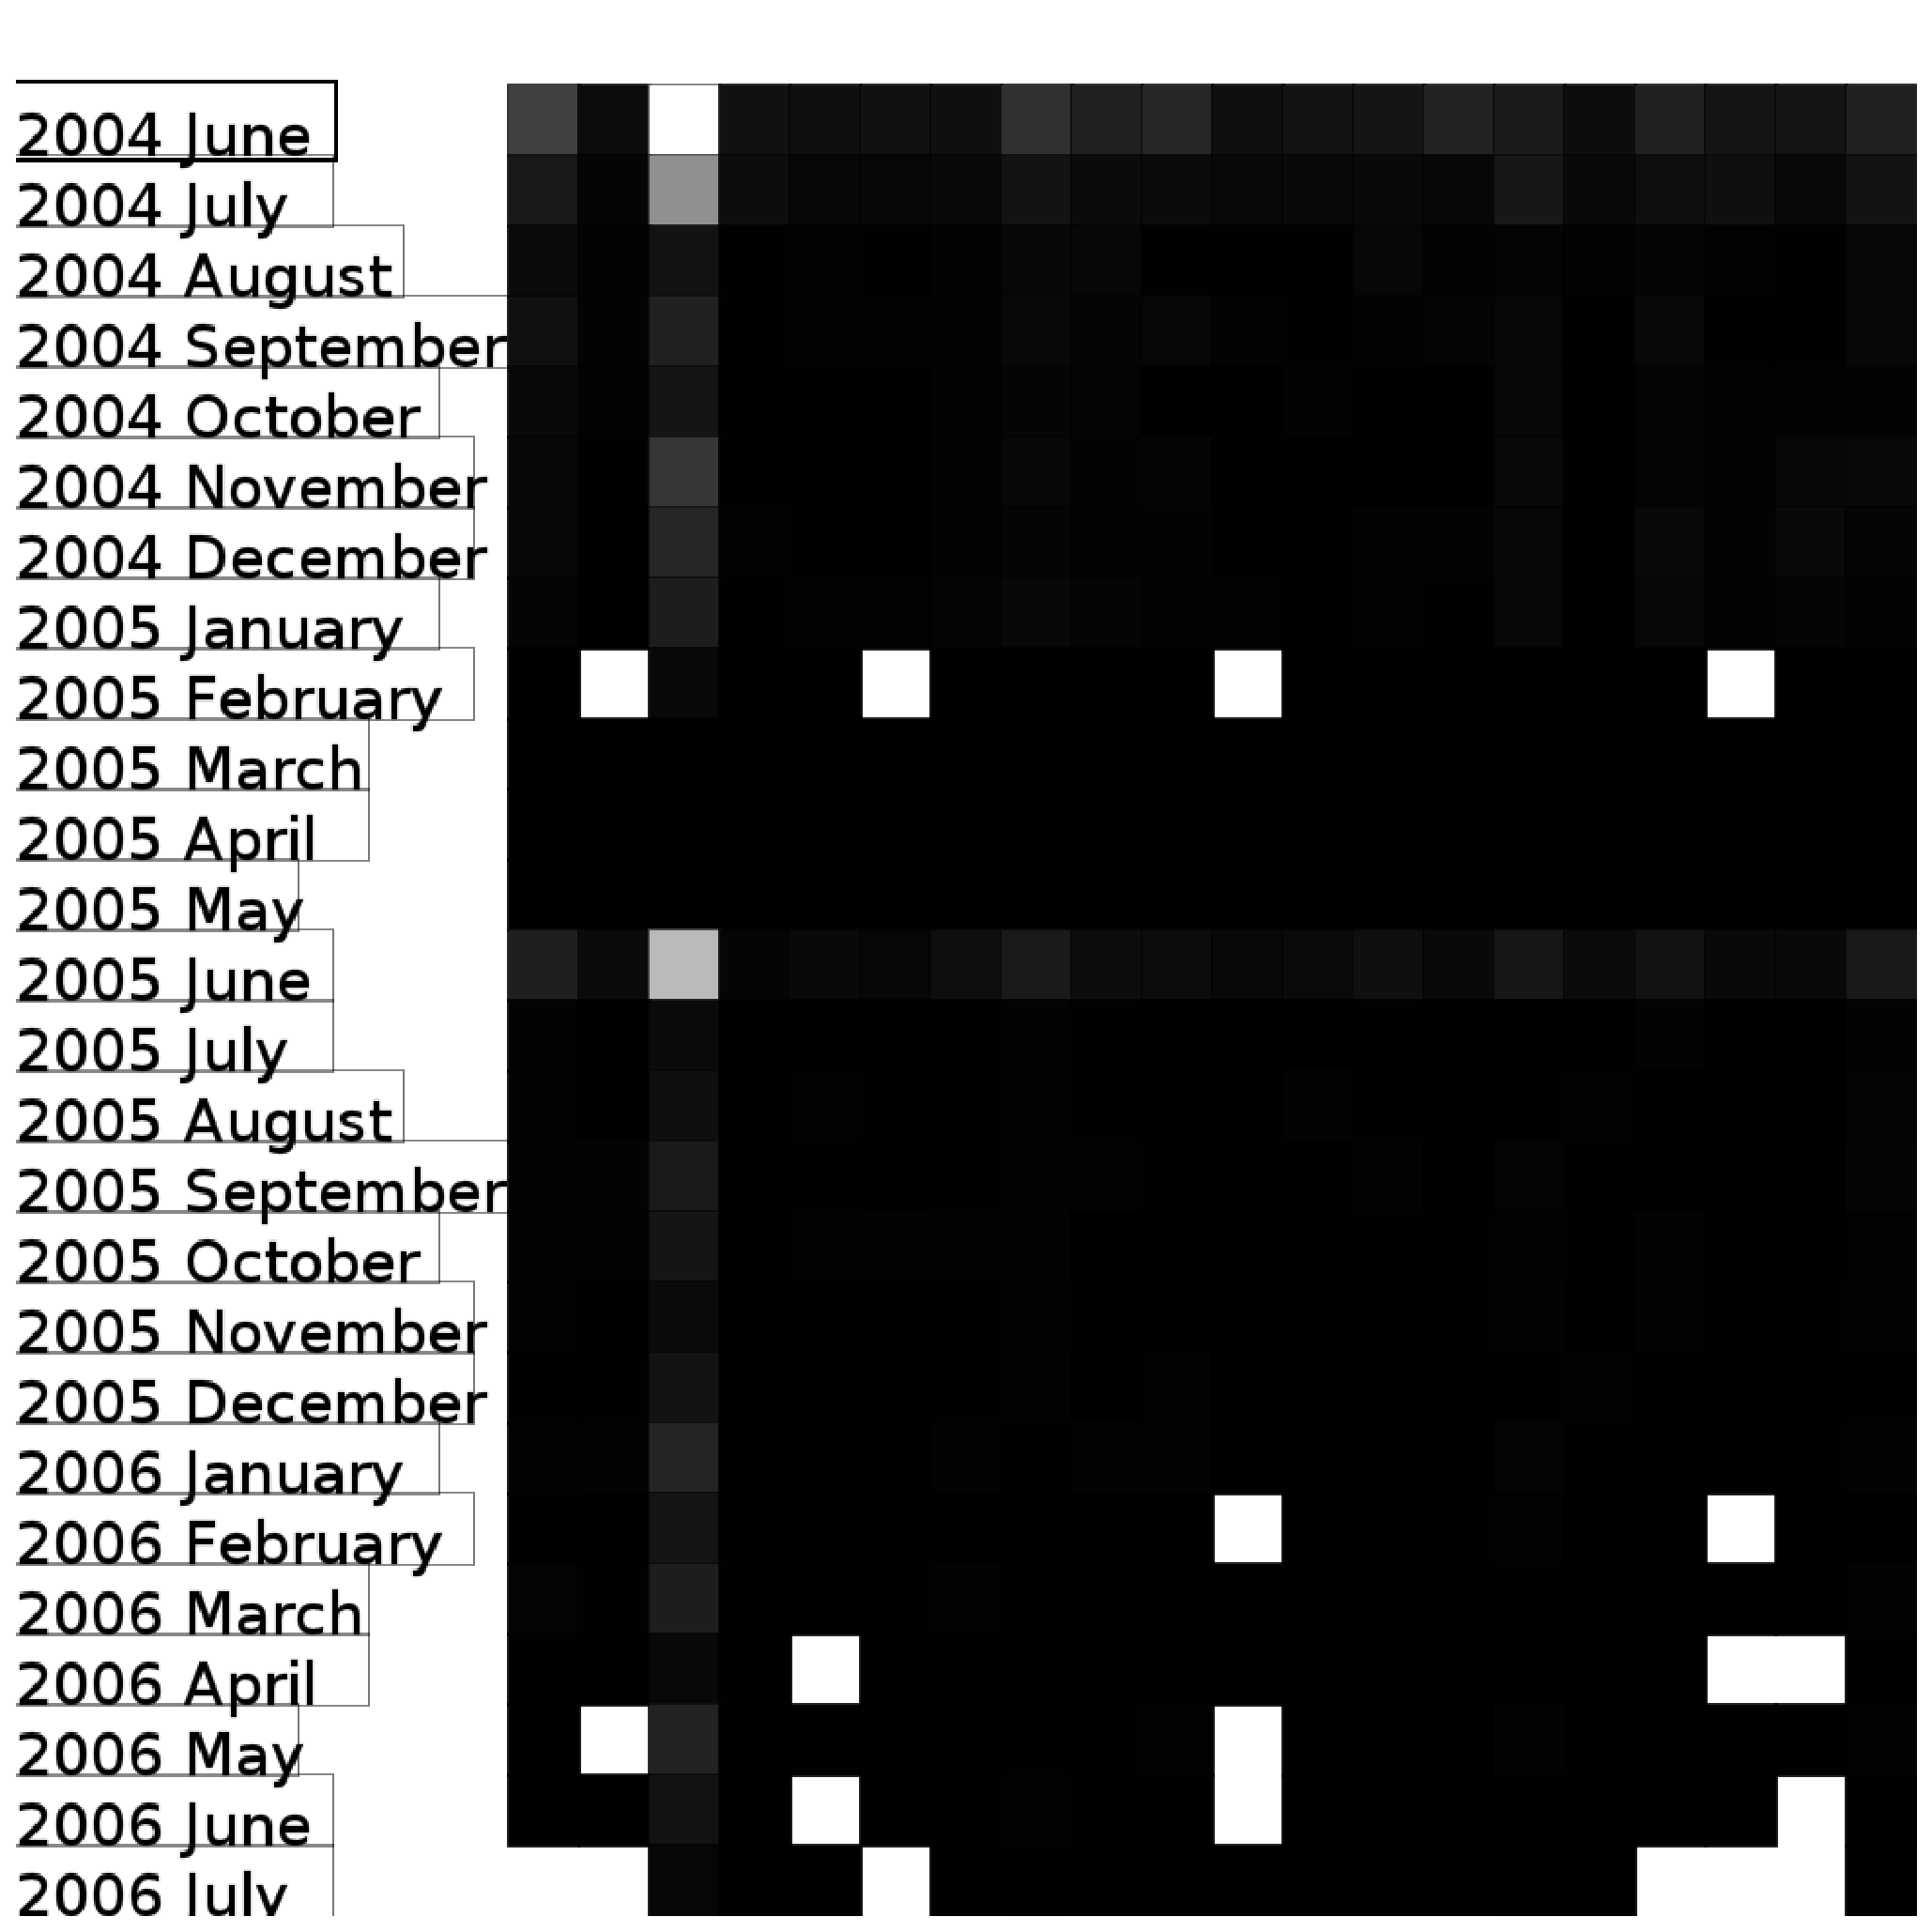
\includegraphics[width=0.45\textwidth]{maxdb7500-everything-by-month}
  \caption{MaxDB 7.500 Topics Analyzed with Static Topic Analysis, 20
    topics over the entire development history of MaxDB 7.500. The
    color of the topic indicates the number of documents matching that
    topic in that month relative to the number of documents (white is
    most, black is least).}
  \label{fig:statictopics}
\end{figure}


%\subsection{Validation}


%   1. well i'm stumped
%   2. look at it?
%   3. investigate those revisions and check the proportion etc
%   4. exploratory
%   5.   work it out
%8.   Validity Threats [0/5]
\section{Validity Threats}

In this study we are explicitly trusting that the programmers annotate
their changes with relevant information. We rely on the descriptions
they provide. If the language of check-in comments was automated we
would only be analyzing that.

We truncated the topics to top 10 tokens, this summary of a topic
might not have been as useful as determining the actual topic distance
between two word topic distributions. By truncating tokens we could be
losing valuable data.

Each project seemed to have their own kind of stop words, we did not
remove them, but perhaps dropping some of these stop words would aid
the clarity of such topic cluster; alternatively it might cause our
topic similarity plots to be fundamentally different. 

The number of
commits per month is inconsistent as some months have a lot of changes
while others months have almost none.
%   1.   validation
%   2.   LDA is questionable
%   3.   blackbox problem
%   4.   not in the token
%   5.   multiple X token
%9.    Future Work

%10.   Conclusions




\section{Conclusions}
%11.   Start file file:/home/abez/projects/lda-paper/lda-paper.tex


%XXX migod comments:

% The first two paras here are good stuff, but I think it belongs in
% section 5 at the end, as a summary of the utility of the approach.
% But can you add more meat to it in terms of numbers?


% In the conclusions you can simply restate what we did and what we
% learned without doing the arguing here.

% The third para is a good one for the conclusions, tho there need to
% be more detail.



% Even with our liberal topic similarity metrics that produced both
% long and short trends, we showed that there are only a few trends in a
% repository which recur. Since so few trends recur and so many
% trends appear only once this suggests that global topic analysis might
% be ignoring locally unique topics. 

% The utility of global topic analysis is questionable if the value of
% information decreases as it becomes older. Perhaps older trends will
% dominate the topic analysis. Windowed localized topic analysis show
% what are the unique topics.

XXX summarize our position

XXX Add more detail here

We presented multiple visualizations that focused on different
aspects of the data: temporality of trends, trend size, and a
condensed overall trend view. The condensed trend view shows much more
information than the views that global analysis could show.


\subsection{ Future Work}

One avenue of future work we think is quite important is automatic
cluster labelling. Given a word distribution we should be able to
automatically select a word or term that best describes that distribution.
Another avenue we wish to investigate the is value of applying
static community-generated software taxonomies to the naming or
grouping of clusters




\bibliographystyle{latex8}
\bibliography{lda-paper}

%\bibliographystyle{abbrv}

% \section{Appendix}

% \begin{itemize}
% \item We are missing a comparison of our technique to the classical technique
% \end{itemize}

\end{document}
